\documentclass[12pt, a4paper]{article}
\usepackage[utf8]{inputenc}
\usepackage[czech]{babel}
\usepackage[left=2.5cm,text={16cm, 24cm},top=3cm]{geometry}
\usepackage{amsmath}
\usepackage{graphicx}
\usepackage{float}
\usepackage{pgfplots}

\begin{document}
\begin{center}
	\begin{huge}\textbf{Bucket Sort}\end{huge} \\
	\vspace{0.4cm}
	Tomáš Blažek (xblaze31) \\
	\textit{PRL - Paralelní a Distribuované algoritmy} \\
	\textit{Fakulta Informačních Technologií, Brno} \\
\end{center}



\section{Rozbor a analýza algoritmu}
\label{sec:rozbor}
Algoritmus bucket sort je řadící algoritmus, který pracuje se s stromem procesorů. Počet použitý procesorů je závislý od počtu řazených prvků $n$. Procesory se dále dělí na listové a nelistové. Množtví použitých listových procesorů $m$ se vypočítá jako $m=log_{2}(n)$, přičemž $m$ se buď rovná k-té mocnině dvou nebo se zarovná na nejbližší vyšší mocninu dvou. Dále pak celkový počet procesorů $p$ v celém stromě procesorů je roven $p = 2m-1$. Algoritmus pracuje na principu, že se rozdělí řazené prvky rovnoměrně mezi jednotlivé listové procesory, přičemž každý listový procesor načítá $n/m$ prvků $(m=log_{2}(n))$ tedy dostaneme časovou složitost $O(n/log_{2}(n))$. Každý listový procesor seřadí svoji posloupnost čísel optimalním sekvenčním algoritmem, tím získáme $O\big(\frac{n}{m}\cdot log_{2}(\frac{n}{m})\big)$ = $O\big(\frac{n}{log_{2}(n)}\cdot log_{2}(log_{2}(n)-log_{2}(log_{2}(n)))\big) = O\big(\frac{n\cdot log_{2}(n)}{log_{2}(n)}-\frac{n\cdot log_{2}(log_{2}(n))}{log_{2}(n)}\big) = O\big(n-\frac{n\cdot log_{2}(log_{2}(n))}{log_{2}(n)}\big)$, což ve výsledku dá $O(n)$. Seřezené posloupnosti zašlou listové procesory svému rodičovskému procesoru a ten obě seřazené posloupnosti spojí do jedné seřazené posloupnosti, tj. $O(n)$. Tento proces se opakuje do té doby než se výsledek propaguje až do kořenového procesoru, to vede na počet iterací  $i = log_{2}(m)-1$. To by ale znamenalo, že by časová složitost byla $O(n.log_{2}(n))$. Musíme ale zohlednit i ten fakt, že v každé iteraci se řadí $n/(2^j)$ prvků pro $j = 1$ až do $j = i$. To nám dává posloupnost $n + \frac{n}{2} + \frac{n}{4} +\frac{n}{8} + ... = 2n$, což patří do $O(n)$. Kořenový procesor následně uloží celou seřazenou posloupnost prvků do paměti $O(n)$. 


\begin{equation}
\begin{split}
\text{Časová složitost: }t(n) &= O(n/log_{2}(n)) + O(n) + O(n) = O(n)\\
\text{Prostorová složitost: }p(n) &= O(log_{2}(n))\\
\text{Celková cena: }c(n) &= O(n) \cdot O(log_{2}(n)) = O(n\cdot log_{2}(n))
\end{split}
\end{equation}

Celková cena algoritmu Bucket Sort je optimální, jelikož odpovídá časové náročnosti optimalního sekvenčního řadícího algoritmu.

\section{Implementace}
Program je implementován v jazyce C++ s využitím knihovny Open MPI. V samotné implementaci programu se jako první operace inicializuje MPI komunikace a zjístí se informace o tom, kolik procesů běží, přičemž si každý proces zjistí svoje identifikační číslo (id). Nejprve kořenový procesor načte obsah vstupního souboru numbers, ze kterého získá řazené prvky a uloží je do paměti. Následně rozešle informace ohledně množství listových procesorů a velikosti kyblíku (bucket), aby listové procesory věděli kolik dat mají přijmout. Dále kořenový procesor rozešle řazené prvky rovnoměrně mezi listové procesory. Ty pomocí funkce \texttt{std::sort} ze standartní knihovny seřadí svoje prvky a uloží je do vektoru. Následně všechny listové procesory pošlou svým rodičovským procesorům svoje seřazené posloupnosti, ty je přijmou, a spojí je do jedné seřazené posloupnoti pomocí knihovní funkce \texttt{std::merge}. Pokud se nejedná o kořenový procesor, tak se proces zaslání seřazených posloupností rodičovskému procesorů a následného spojení opakuje do té doby, dokud se posloupnost nedostane do kořenového procesoru, kde se po spojení nachází již celá seřazená posloupnost prvků. Kořenový procesor následně vypíše prvky na standartní výstup (stdout).

\section{Experimenty}
Nad implementovaným algoritmem byly prováděny experimenty v podobě opakovaného spouštění řazení s konstantním krokem 5 tisíc v rozsahu od 0 do 60 tisíc prvků a byla měřena doba za níž algoritmus dokončí svůj výpočet. Časové hodnoty byly získány za pomoci funkce přímo z knihovny Open MPI, která vrací čas v sekundách, ale kvůli lepší vizualizaci jsou hodnoty v grafu převedeny na milisekundy. Časové údaje byly při experimentu měřeny pouze pro samotný algoritmus, tedy bylo z měření vynecháno načítání prvků ze souboru a konečný tisk výsledku na standartní výstup.


\begin{figure}[h]\centering
	\label{fig:experimenty}
	\begin{tikzpicture}
		\begin{axis}[
			xlabel={Počet prvků} width={1.8\textwidth} style={/pgf/number format/fixed},
			ylabel=Čas (ms)]
		\addplot coordinates {	
			(0,0)
			(5000,3.826)
			(10000,5.139)
			(15000,6.912)
			(20000,9.510)
			(25000,10.709)
			(30000,12.555)
			(35000,13.900)
			(40000,14.654)
			(45000,16.437)
			(50000,19.205)
			(55000,20.180)
			(60000,23.636)
		};
		\end{axis}
	\end{tikzpicture}
	\caption{Graf výsledku experimentů časové náročnosti}	
\end{figure}

\section{Komunikační protokol}
Komunikační protokol je znázorněný pomocí sekvenčního diagramu. Ten popisuje komunikaci mezi jednotlivými procesory, které by se dali rozdělit do tří skupin. Do první skupiny patří pouze kořenový procesor a do zbylých dvou skupin se řadí procesory listové a nelistové. V diagramu jsou tedy uvedeny pouze tyto tři skupiny, aby popis mohl být obecný pro libovolný počet procesorů s výjimkou použití jednoho procesoru. To je z důvodu toho, že při použití pouze jednoho procesoru neprobíhá žádná komunikace a výsledek je rovnou uložen v paměti kořenového procesoru. Proměnné použité v diagramu jsou definovány v kapitole \ref{sec:rozbor}.

\begin{figure}[H]
	\centering
	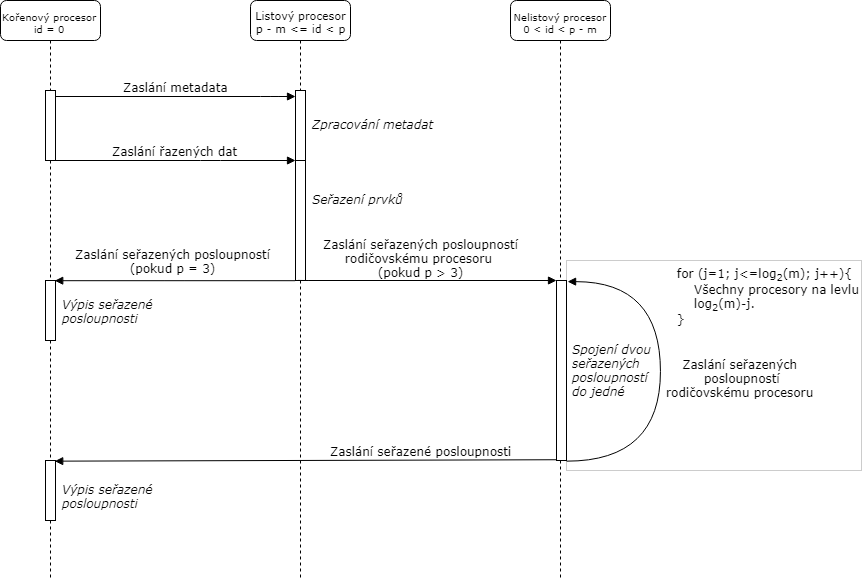
\includegraphics[scale=0.53]{pics/seq.png}
	\caption{Sekvenční diagram komunikace procesorů}	
\end{figure}


\section{Závěr}
V kapitole experimentů z grafu plyne, že algoritmus má lineární časový průběh, což potvrzuje odhad časové složitosti z rozboru a analýzy algoritmu, který byl určen jako $O(n)$. Experimenty byly prováděny na školním serveru Merlin s operačním systémem CentOS.
\end{document}